\themaM
\graphicspath{{../../S13_Perimetres_et_aires/Images/}}

\chapter{Périmètres et aires}
\label{S13}

%Piece de curvica
\newcommand{\vg}{\psarc(3,0){2.24}{153.4}{-153.4}}
\newcommand{\vm}{\psline(1,-1)(1,1)}
\newcommand{\vd}{\psarc(-1,0){2.24}{-26.6}{26.6}}
\newcommand{\hb}{\psarc(0,3){2.24}{-116.6}{-63.4}}
\newcommand{\hm}{\psline(-1,1)(1,1)}
\newcommand{\hh}{\psarc(0,-1){2.24}{63.4}{116.6}}
 \newcommand{\curvica}[5]{\rput(#1,#2){#3} \rput(#1,#2){#4} \rput(#1,#2){\large #5}}  

%%%%%%%%%%%%%%%%%%%%%%%%%%%%%%%
%%%%%%%%%%%%%%%%%%%%%%%%%%%%%%%%
\begin{autoeval}
   \small
   \begin{enumerate}
      \item Il calcule le périmètre et l’aire des figures usuelles (rectangle, triangle, disque).
      \item Il calcule le périmètre et l’aire d’un assemblage de figures.
      \item Il vérifie la cohérence des résultats du point de vue des unités (adaptées) pour les calculs de longueurs et d’aires.
      \item Il effectue des conversions d’unités de longueurs et d’aires.
   \end{enumerate}
\end{autoeval}

\begin{prerequis}
   \begin{itemize}
      \item[\com] Mener des calculs impliquant des grandeurs mesurables, exprimer les résultats dans les unités adaptées.
      \item[\com] Vérifier la cohérence des résultats des unités.
      \item[\com] Effectuer des conversions d’unités.
   \end{itemize}
\end{prerequis}

\vfill

\begin{debat}[Haïku]
   Un haïku est un petit poème traditionnel japonais, de forme très concise (dix-sept syllabes en trois vers : 5-7-5 ou 7-5-5 ou 5-5-7). {\it Richard Cauche} est enseignant de mathématiques et membre de l’IREM de Paris. Il nous fait partager ces haïkus mathématiques sur le périmètre et l'aire du disque :
   \begin{center}
      
\includegraphics[height=6cm]{circonference}
      \hspace{10mm}
      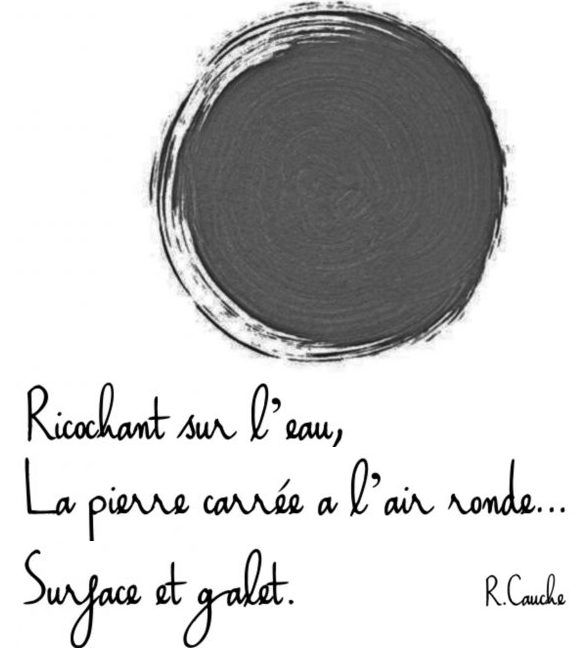
\includegraphics[height=6cm]{surface}
   \end{center}
   \begin{cadre}[B2][J4]
      \begin{center}
         Vidéo : \href{https://www.yout-ube.com/watch?v=TcNfC8b4hUg}{\bf Archimède et le nombre $\pi$}, chaîne YouTube {\it m@ths et tiques}, Yvan Monka.
      \end{center}
   \end{cadre}
\end{debat}



%%%%%%%%%%%%%%%%%%%%%%%%%%%%%%%%%%%%
%%%%%%%%%%%%%%%%%%%%%%%%%%%%%%%%%%%%
\activites

\begin{activite}[Une aire multiforme]
   {\bf Objectifs :} différencier périmètre et aire ; comparer des périmètres et des aires sans utiliser la mesure.

   \begin{QCM}
      Le curvica est un jeu-puzzle de 24 pièces inventé par {\bf Jean Fromentin} en 1982 afin de travailler sur les notions de périmètre, d’aire et de symétrie, entre autres ! À partir d’un carré, on obtient une pièce du puzzle curvica en \og creusant \fg, en \og bombant \fg ou en laissant droits les côtés. Les arcs produits sont tous identiques.
      
      \begin{center}
         \begin{pspicture}(0,0)(12,8)
            \psline(0,8)(0,0)(12,0)
            \curvica{1}{1}{\hm}{\vg}{K} \curvica{3}{1}{\hm}{\vd}{T} \curvica{5}{1}{\hb}{\vd}{W} \curvica{7}{1}{\hh}{\vg}{V} \curvica{9}{1}{\hb}{\vd}{N} \curvica{11}{1}{\hb}{\vm}{E} %ligne 1
            \curvica{1}{3}{\hb}{\vd}{H} \curvica{3}{3}{\hm}{\vd}{F} \curvica{5}{3}{\hb}{\vg}{R} \curvica{7}{3}{\hb}{\vd}{L} \curvica{9}{3}{\hh}{\vd}{C} \curvica{11}{3}{\hb}{\vm}{X} %ligne 2
            \curvica{1}{5}{\hm}{\vd}{U} \curvica{3}{5}{\hm}{\vg}{D} \curvica{5}{5}{\hh}{\vd}{A} \curvica{7}{5}{\hb}{\vd}{M} \curvica{9}{5}{\hb}{\vg}{Q} \curvica{11}{5}{\hb}{\vm}{O} %ligne 3
            \curvica{1}{7}{\hm}{\vm}{I} \curvica{3}{7}{\hm}{\vd}{J} \curvica{5}{7}{\hm}{\vg}{S} \curvica{7}{7}{\hm}{\vg}{P} \curvica{9}{7}{\hm}{\vd}{B} \curvica{11}{7}{\hm}{\vm}{G} %ligne 4
         \end{pspicture}
      \end{center}
      \vspace*{-10mm}
      
      \begin{spacing}{1.5}
      \begin{enumerate}
         \item On s’intéresse uniquement aux pièces A, B, C, D, E et F que l'on pourra colorier.
            \begin{enumerate}
               \item Classer ces six pièces du plus petit au plus grand périmètre. \pointilles
               \item Classer ces six pièces de la plus petite à la plus grande aire. \pointilles
               \item Quelles sont les deux pièces qui ont la même aire et le même périmètre ? \pointilles
               \item Trouver deux pièces qui ont le même périmètre, mais des aires différentes. \pointilles 
            \end{enumerate}
         \item On s'intéresse maintenant à toutes les pièces.
            \begin{enumerate}
               \item Y a-t-il une unique pièce d’aire minimale ? \pointilles
               \item Y a-t-il une unique pièce de périmètre minimum ? \pointilles             
               \item Y a-t-il une unique pièce d’aire maximale ? \pointilles           
               \item Y a-t-il une unique pièce de périmètre maximum ? \pointilles         
               \item Y a-t-il une ou des pièces de même aire que la carré I ? \pointilles
               \item Y a-t-il une ou des pièces de même périmètre que la carré I ? \pointilles \\ [-15mm]
            \end{enumerate}
      \end{enumerate}
      \end{spacing}
   \end{QCM}
\end{activite}

\vfill\hfill{\small\it Source : \href{https://irem.univ-reunion.fr/spip.php?article802}{Curvica - activités mathématiques ludiques}, Yves Martin, IREM de la Réunion.}


%%%%%%%%%%%%%%%%%%%%%%%%%%%%%%%%%%%
%%%%%%%%%%%%%%%%%%%%%%%%%%%%%%%%%%%
\cours 

%%%%%%%%%%%%
\section{Périmètres et aires usuelles}

$\bullet$ Le périmètre d'un polygone est la somme des longueurs des segments qui le compose ; \\
$\bullet$ la circonférence d'un cercle de rayon $r$ se calcule grâce à la formule $\mathcal{p} =2\times\pi\times r$. \medskip

Pour les aires, on a les formules suivantes : \\ [-2mm]
\begin{minipage}[t]{5cm}
   \Formule[Aire,Surface=rectangle,Ancre={(2.5,-2)},Couleur=yellow!10]
\end{minipage}
\qquad
\begin{minipage}[t]{5cm}
   \Formule[Aire,Surface=triangle,Ancre={(2.5,-2)},Couleur=yellow!10]
\end{minipage}
\qquad
\begin{minipage}[t]{5cm}
   \Formule[Aire,Surface=disque,Ancre={(2.5,-2)},Couleur=yellow!10]
\end{minipage}

\vspace*{40mm}

\hspace*{-11mm}
\begin{minipage}[t]{5cm}
   \begin{exemple}[1.5]
      Aire d'un rectangle de longueur \udm{0,3} et de largeur \udm{0,2} : \\ [1mm]
      $\udm{0,3}\times\udm{0,2} =\udmq{0,06}$.
   \end{exemple}
\end{minipage}
\qquad
\begin{minipage}[t]{5cm}
   \begin{exemple}[1.5]
      Aire d'un triangle de base \umm{28} et de hauteur relative \umm{13} : \\ [2mm]
   $\dfrac{\umm{28}\times\umm{13}}{2} =\ummq{182}$.
   \end{exemple}
\end{minipage}
\qquad
\begin{minipage}[t]{5cm}
   \begin{exemple}[1.5]
      Aire et périmètre d'un disque de rayon \ucm{1,2} : \\
      $\mathcal{A} =\pi\times(\ucm{1,2})^2\approx\ucmq{4,52}$. \\
      $\mathcal{P} =2\times\pi\times(\ucm{1,2})\approx\ucm{7,54}$.
   \end{exemple}
\end{minipage}

\begin{remarque}
   pour calculer l'aire d'une figure complexe, il suffit de la \og découper \fg{} en figures usuelles et d'additionner ou de soustraire les aires qui la constituent.
\end{remarque}


%%%%%%%%%%%   
\section{Conversions}

On peut mesurer une longueur grâce au mètre (m) et ses multiples et sous-multiples :

\Tableau[Metre,FlechesH]{7321/3}
\vspace*{-8mm}

\begin{exemple*1}
   $\ukm{0,07321} =\udam{7,321} =\um{73,21}=\udm{732,1} =\ucm{7321} =\umm{73210}$. 
\end{exemple*1}

\bigskip

L'aire est une grandeur composée, correspondant au produit de deux longueurs. Chaque unité d'aire dans le tableau comporte donc deux colonnes. Pour désigner une aire, on utilise le mètre carré (\umq{}) et ses multiples et sous-multiples. \\
Pour les mesures agraires, on utilise l'are (a) qui équivaut à \umq{100} et l'hectare (ha) qui vaut 100 ares. \smallskip

\Tableau[Carre,Colonnes,Are,FlechesH]{3701/4}
\vspace*{-8mm}

\begin{exemple*1}
   \ukmq{0,03701} = \uha{3,701} = \uhmq{3,701} = \ua{370,1} = \umq{37010} = \udmq{3701000}\dots
\end{exemple*1}


%%%%%%%%%%%%%%%%%%%%%%%%%%%%%%
%%%%%%%%%%%%%%%%%%%%%%%%%%%%%%
\exercicesbase

\begin{colonne*exercice}

\begin{exercice} %1
   Effectuer les conversions de longueurs suivantes :
   \begin{enumerate}
      \item $\um{1275} =\pointilles \ucm{}$
      \item $\udm{32,5} =\pointilles \udam{}$
      \item $\ucm{345697,34} =\pointilles \ukm{}$
      \item $\um{0,003} =\pointilles \umm{}$
      \item $\ukm{2,5} =\pointilles \um{}$
   \end{enumerate}
\end{exercice}

\begin{corrige}
   \ \\ [-5mm]
   \begin{enumerate}
      \item $\um{1275} =\blue\ucm{127500}$
      \item $\udm{32,5} =\blue\udam{0,325}$
      \item $\ucm{345697,34} =\blue\ukm{3,4569734}$
      \item $\um{0,003} =\blue\umm{3}$
      \item $\ukm{2,5} =\blue\um{2500}$
   \end{enumerate}
\end{corrige}

\medskip


\begin{exercice} %2
   Effectuer les conversions d'aires suivantes :
   \begin{enumerate}
      \item $\umq{1275} =\pointilles \ucmq{}$
      \item $\udmq{32,5} =\pointilles\udamq{}$
      \item $\ucmq{345697,34} =\pointilles\umq{}$
      \item $\umq{0,003} =\pointilles\ummq{}$
      \item $\ukmq{2,5} =\pointilles \umq{}$
   \end{enumerate}
\end{exercice}

\begin{corrige}
\ \\ [-5mm]
   \begin{enumerate}
      \item $\umq{1275} =\blue\ucmq{12750000}$
      \item $\udmq{32,5} =\blue\udamq{0,00325}$
      \item $\ucmq{345697,34} =\blue\umq{34,569734}$
      \item $\umq{0,003} =\blue\ummq{3000}$
      \item $\ukmq{2,5} =\blue\umq{2500000}$
   \end{enumerate}
\end{corrige}

\medskip


\begin{exercice} %3
   Donner une unité de mesure usuelle pour chacun des objets suivants :
   \begin{enumerate}
      \item Longueur d'une piste d'athlétisme.
      \item Surface d'un jardin.
      \item Longueur d'une fourmi.
      \item Surface d'une feuille.
      \item Largeur d'une chambre.
      \item Surface d'un champ.
      \item Rayon d'une planète.
   \end{enumerate}
\end{exercice}

\begin{corrige}
\ \\ [-5mm]
   \begin{enumerate}
      \item La longueur d'une piste d'athlétisme se mesure généralement en {\blue mètres}.
      \item La surface d'un jardin  se mesure généralement en {\blue mètres carrés} ou en {\blue ares}.
      \item La longueur d'une fourmi se mesure généralement en {\blue millimètres}.
      \item La surface d'une feuille se mesure généralement en {\blue centimètres carrés}.
      \item La largeur d'une chambre se mesure généralement en {\blue mètres}.
      \item La surface d'un champ se mesure généralement en {\blue hectares}.
      \item Le rayon d'une planète se mesure généralement en {\blue kilomètres}.
   \end{enumerate}
\end{corrige}

\medskip


\begin{exercice} %4
   Sachant que l'unité d'aire est le carreau ($u.a.$), déterminer l'aire de chaque surface suivante.
   \begin{center}
      {\psset{unit=0.5}
      \begin{pspicture}(0,-4.5)(15,10)
         \psgrid[subgriddiv=0,gridlabels=0,gridcolor=lightgray](0,-5)(15,10)
         \psset{linewidth=0.3mm}
         \psframe(1,1)(4,3)
         \rput(2.5,2.5){\ding{202}}
         \pspolygon(5,0)(11,0)(10,4)(8,4)(5,2)
         \rput(8.5,1.5){\ding{205}}
         \pspolygon(1,4)(1,9)(5,9)(5,8)(2,8)(2,7)(4,7)(4,6)(2,6)(2,4)
         \rput(1.5,6.5){\ding{203}}
         \pspolygon(6,7)(12,9)(6,9)
         \rput(7.5,8.4){\ding{204}}
         \pspolygon(5,4)(5,6)(12,6)(12,8)(14,8)(14,4)(13,3)(14,2)(14,1)(12,1)(11,3)(12,5)(6,5)
         \rput(12.5,5.5){\ding{206}}
         \psline(3,-2)(1,-2)(1,-4)(2,-4)
         \psarc(3,-4){1}{0}{180}
         \psline(4,-4)(6,-4)(6,-2)(5,-2)
         \psarc(4,-2){1}{0}{180}
         \rput(3.5,-2.5){\ding{207}} 
         \psline(7,-1)(14,-1)
         \psline(7,-4)(14,-4)
         \psline(8,-2)(8,-3)
         \psline(13,-2)(13,-3)
         \psarc(8,-4){1}{90}{180}
         \psarc(8,-1){1}{180}{-90}
         \psarc(13,-4){1}{0}{90}
         \psarc(13,-1){1}{-90}{0}
         \pscircle(10,-2.5){1}
         \rput(11.5,-2.5){\ding{208}}
         \psframe[fillstyle=solid,fillcolor=gray](14,9)(15,10)
         \rput(13.25,9.5){$u.a.$}
      \end{pspicture}}
   \end{center}
\end{exercice}

\begin{corrige}
   On peut par exemple procéder par découpage et recollement pour obtenir des unités entières. \\
   \begin{enumerate}
      \item La surface 1 mesure {\blue 6 $u.a.$}
      \item La surface 2 mesure  {\blue 10 $u.a.$}
      \item La surface 3 mesure {\blue 6 $u.a.$}
      \item La surface 4 mesure {\blue 19 $u.a.$}
      \item La surface 5 mesure {\blue 22,5 $u.a.$}
      \item La surface 6 mesure {\blue 10 $u.a.$}
      \item La surface 7 mesure {\blue 15 $u.a.$}
   \end{enumerate}
\end{corrige}

\medskip


\begin{exercice} %5
   Résoudre les petits problèmes suivants :
   \begin{enumerate}
      \item Quelle est l'aire d'un carré de périmètre \ucm{32} ?
      \item Quel est le périmètre d'un rectangle de largeur \um{6} et d'aire \umq{48} ?
   \end{enumerate}
\end{exercice}

\begin{corrige}
   \ \\ [-5mm]
   \begin{enumerate}
      \item Le périmètre d'un carré vaut $4\times c$, donc $c =\ucm{32}\div4 =\ucm{8}$. \\
         L'aire du carré vaut $(\ucm{8})^2 =\blue\ucmq{64}$.
      \item L'aire d'un rectangle vaut $L\times\ell$. \\
         On a alors $L\times\um{6} =\umq{48}$ soit $L =\dfrac{\umq{48}}{\um{6}} =\um{8}$. \\ [1mm]
         Donc, le périmètre vaut $2\times(\um{8}+\um{6}) =\blue\um{28}$.
   \end{enumerate}
\end{corrige}

\medskip


\begin{exercice} %6
   Calculer l'aire et le périmètre de ces figures. \\
   {\psset{unit=0.45}
   \small
   \begin{pspicture}(-1,0)(13,6)
      \psframe(1,1)(7,5)
      \psframe(1,1)(1.4,1.4)
      \rput(4,1){/\!\!/}
      \rput(4,5){/\!\!/}
      \rput(1,3){$\times$}
      \rput(7,3){$\times$}
      \rput(4,0.2){\um{8}}
      \rput{90}(0.2,2.7){\um{4,5}}
      \rput(4,3){A}
      
      \psframe(10,1)(13,4)
      \psframe(10,1)(10.4,1.4)
      \rput(11.5,1){$\bullet$}
      \rput(11.5,4){$\bullet$}
      \rput(10,2.5){$\bullet$}
      \rput(13,2.5){$\bullet$}
      \rput(11.5,0.2){\umm{12,3}}
      \rput(11.5,2.5){B}
   \end{pspicture} \\

   \begin{pspicture}(-1,0)(13,5)
      \pspolygon(1,1)(7,1)(2,5)
      \psframe(2,1)(2.3,1.3)
      \psline(2,1)(2,5)
      \rput{-40}(5.2,3.5){\ucm{6,9}}
      \rput{78}(0.8,3.2){\ucm{4,6}}
      \rput(3.5,0){\ucm{6,6}}
      \rput{90}(2.5,2.7){\ucm{4,4}}
      \rput(3.8,2.2){C}
      
      \pspolygon(9,1)(14,1)(14,6)
      \psframe(14,1)(13.7,1.3)
      \rput(11.5,0){\ukm{8,5}}
      \rput{45}(11.3,4){\ukm{12,5}}
      \rput(11.5,1){|\!\!|}
      \rput(14,3.5){=}
      \rput(12.5,2.5){D}
   \end{pspicture} \\
   
   \begin{pspicture}(-1,1)(13,5.5)
      \pscircle(3,3){2.5}
      \psline(3,3)(5.5,3)
      \rput(4.25,2.5){\udm{1,5}}
      \rput(3,3.75){E}
      \pscircle(12,3){2}
      \psline(10,3)(14,3)
      \rput(12,2.5){\um{5,6}}
      \rput(12,3.5){F}
   \end{pspicture}}
\end{exercice}

\begin{corrige}
   \textcolor{G1}{$\bullet$} Figure A : on a un rectangle de côtés \um{8} et \um{4,5}. \\
      $\mathcal{P} =2\times(L+\ell) =2\times(\um{8}+\um{4,5}) =\blue\um{25}$. \\
      $\mathcal{A} =L\times\ell =\um{8}\times\um{4,5} =\blue\umq{36}$. \\
   \textcolor{G1}{$\bullet$} Figure B : on a un carré de côté \umm{12,3}. \\
      $\mathcal{P} =4\times c =4\times\umm{12,3} =\blue\umm{49,2}$. \\ 
      $\mathcal{A} =c\times c =\umm{12,3}\times\umm{12,3} =\blue\ummq{151,29}$. \\ 
   \textcolor{G1}{$\bullet$} Figure C : on a un triangle de base \ucm{6,6} et de hauteur associée \ucm{4,4}. \\
      $\mathcal{P} =\ucm{6,6}+\ucm{6,9}+\ucm{4,6} =\blue \ucm{18,1}$. \\ [1mm]
      $\mathcal{A} =\dfrac{b\times h}{2} =\dfrac{\ucm{6,6}\times\ucm{4,4}}{2}=\blue \ucmq{14,52}$. \\ [1mm]
   \textcolor{G1}{$\bullet$} Figure D : on a un triangle de base \ukm{8,5} et de hauteur associée \ukm{8,5}. \\
      $\mathcal{P} =2\times\ukm{8,5}+\ukm{12} =\blue \ukm{29}$. \\ [1mm]
      $\mathcal{A} =\dfrac{b\times h}{2}  =\dfrac{\ukm{8,5}\times\ukm{8,5}}{2}=\blue \ukmq{36,125}$. \\ [1mm]
   \textcolor{G1}{$\bullet$}  Figure E : on a un disque de rayon \udm{1,5}. \\
      $\mathcal{P} =2\times\pi\times r =2\times\pi\times\udm{1,5} \approx\blue \udm{9,42}$. \\
      $\mathcal{A} =\pi\times r^2 =\pi\times(\udm{1,5})^2 \approx\blue \udmq{7,07}$. \\
   \textcolor{G1}{$\bullet$}  Figure F : on a un disque de rayon \um{2,8}. \\
      $\mathcal{P} =2\times\pi\times r =2\times\pi\times\um{2,8} \approx\blue \um{17,59}$. \\
      $\mathcal{A} =\pi\times r^2 =\pi\times(\um{2,8})^2 \approx\blue \umq{24,63}$. \\       
\end{corrige}

\medskip


\begin{exercice} %7
   L'unité d'aire est le carré.
   \begin{enumerate}
      \item On peut regrouper les surfaces ci-dessous par deux ou par trois sauf une, laquelle ?
      \item Calculer alors l'aire de chaque surface.
   \end{enumerate}
   \begin{center}
      {\psset{unit=0.65}
      \small
      \begin{pspicture}(0,4.5)(11,12.8)
         \psgrid[subgriddiv=0,gridlabels=0,gridcolor=lightgray](0,4)(11,13)
         \psset{fillstyle=solid,fillcolor=lightgray}
         
         \pscustom{\psarc(2,11){1}{0}{180} \psarcn(1,10){1}{90}{0} \psarcn(3,10){1}{180}{90}}
         \rput(2,11.25){\small A}
         \pscustom{\psarc(5,11){1}{0}{180} \psline(4,11)(4,10) \psarc(4,11){1}{270}{0} \psarc(6,11){1}{180}{270} \psline(6,10)(6,11)}
         \rput(5,11.5){\small B}
         \pscircle(8,11){1}
         \rput(8,11){\small C}
         
         \pscustom{\psarc(2,8){1}{90}{180} \psarcn(1,7){1}{90}{0} \psarc(2,8){1}{270}{0} \psarcn(3,9){1}{270}{180}}
         \rput(2,8){\small D}
         \pscustom{\psarc(5,8){1}{180}{0} \psline(6,8)(7,8) \psarc(6,8){1}{0}{180} \psline(5,8)(4,8)}
         \rput(5.5,8){\small E}
         \pscustom{\psarcn(8,7){1}{90}{0} \psarcn(10,7){1}{180}{90} \psarcn(10,9){1}{270}{180} \psarcn(8,9){1}{0}{270}}
         \rput(9,8){\small F}  
         
         \pscustom{\psline(1,5)(1,6)(3,6) \psarcn(3,5){1}{90}{0} \psline(4,5)(2,5)(2,4) \psarc(1,4){1}{0}{90}}
         \rput(2.5,5.5){\small G}
         \pscustom{\psarc(6,5){1}{90}{180} \psarcn(5,4){1}{90}{0} \psline(6,4)(6,5)(7,5)(7,4) \psarcn(8,4){1}{180}{90} \psarc(7,5){1}{0}{90} \psline(7,6)(6,6)}
         \rput(6.5,5.5){\small H}
           
      \end{pspicture}}
   \end{center}
\end{exercice}

\begin{corrige}
\ \\ [-5mm]
   \begin{enumerate}
      \item On peut regrouper A et D ; B, C et E ; G et H. \\
         {\blue La surface Fest seule}. \smallskip
      \item \textcolor{G1}{$\bullet$} Les figures A et D peuvent être vues comme un rectangle de mesures $2u$ et $u$, leur aire vaut {\blue $2u^2$}. \\
         \textcolor{G1}{$\bullet$} Les figures B, C et E peuvent être recomposées en un disque de rayon $u$, leur aire veut {\blue $\pi u^2$}. \\
         \textcolor{G1}{$\bullet$} Les figures G et H peuvent être recomposées en un rectangle de mesures $3u$ et $u$, leur aire veut {\blue $3u^2$}. \\
         \textcolor{G1}{$\bullet$} La figure F peut être vue comme un carré de côté $2u$ auquel on enlève quatre quarts de disque, soit un disque de rayon $u$. $\mathcal{A} =\blue 4u^2-\pi u^2$.
   \end{enumerate}
\end{corrige}

\medskip


\begin{exercice} %8
   Dans cette figure, on a : \\
   \begin{minipage}{2cm}
      $AB =\ucm{9}$ \\
      $BC =\ucm{21}$ \\
      $CD =\ucm{11}$ \\ 
      $DE =\ucm{9}$ \\
      $EF =\ucm{11}$ \\
      $GH =\ucm{7}$
   \end{minipage}
   \qquad
   \begin{minipage}{5cm}
   {\psset{unit=1.3}
      \small
      \begin{pspicture}(-0.5,-0.3)(3.5,2.5)
         \psframe(0,0)(3,2)
         \pspolygon(2,0)(3,1)(1,2)(0,0.8)
         \rput(-0.2,-0.2){$G$}
         \rput(-0.2,2.2){$A$}
         \rput(3.2,-0.2){$E$}
         \rput(3.2,2.2){$C$}
         \rput(2,-0.2){$F$}
         \rput(3.2,1){$D$}
         \rput(1,2.2){$B$}
         \rput(-0.2,0.8){$H$}
      \end{pspicture}}
   \end{minipage} \\
   \begin{enumerate}
      \item Calculer le périmètre du rectangle $ACEG$.
      \item Calculer l'aire du quadrilatère $BDFH$.
   \end{enumerate}
\end{exercice}

\begin{corrige}
   \ \\ [-5mm]
   \begin{enumerate}
      \item $\mathcal{P}_{ACEG} =2\times(AC+CE)$. \\
         Or, $AC =AB+BC =\ucm{9}+\ucm{21} =\ucm{30}$ ;\\
         et $CE =CD+DE =\ucm{11}+\ucm{9} =\ucm{20}$. \\
         D'où $\mathcal{P}_{ACEG} =2\times(\ucm{30}+\ucm{20}) =\ucm{100}$. \\
         {\blue Le périmètre du rectangle $ACEG$ est de \ucm{100}}.
      \item Pour calculer l'aire du quadrilatère $BDFH$, on calcule l'aire du rectangle $ACEG$ auquel on soustrait l'aire de chacun des triangles rectangles $ABH$, $BCD$, $DEF$ et $FGH$. \\
      $\mathcal{A}_{ACEG} =AC\times CE =\ucm{30}\times\ucm{20} =\ucmq{600}$. \\ [1.5mm]
      $\mathcal{A}_{ABH} =\dfrac{HA\times AB}{2} =\dfrac{\ucm{13}\times\ucm{9}}{2} =\ucmq{58,5}$. \\ [1.5mm]
      $\mathcal{A}_{BCD} =\dfrac{BC\times CD}{2} =\dfrac{\ucm{21}\times\ucm{11}}{2} =\ucmq{115,5}$. \\ [1.5mm]
      $\mathcal{A}_{DEF} =\dfrac{DE\times EF}{2} =\dfrac{\ucm{9}\times\ucm{11}}{2} =\ucmq{49,5}$. \\ [1mm]
      $\mathcal{A}_{FGH} = \dfrac{FG\times GH}{2} =\dfrac{\ucm{19}\times\ucm{7}}{2} =\ucmq{66,5}$. \\ [1.5mm]
      $\mathcal{A}_{BDFH} =\ucmq{600}-\ucmq{58,5}-\ucmq{115,5}$ \\
      \hspace*{14mm} $-\ucmq{49,5}-\ucmq{66,5} =\ucmq{310}$. \\
      {\blue L'aire du quadrilatère $BDFH$ est de \ucmq{310}}.
   \end{enumerate}
\end{corrige}

\end{colonne*exercice}


%%%%%%%%%%%%%%%%%%%%%%%%%%%%%%%
%%%%%%%%%%%%%%%%%%%%%%%%%%%%%%%
\Recreation


\begin{enigme}[Tel père, tel fils]

\medskip

C’est l’histoire d’un petit rectangle de dimensions $\umm{2}\times\umm{3}$. \\
   Chaque jour, il s’agrandit pour devenir un rectangle plus grand : sa nouvelle largeur est égale à son ancienne longueur ; sa nouvelle longueur est égale à la somme de ses deux anciennes dimensions. \\
   
   {\bf Au bout de combien de jours son aire dépassera-t-elle \umq{1,5} ?} \\

   \begin{center}
      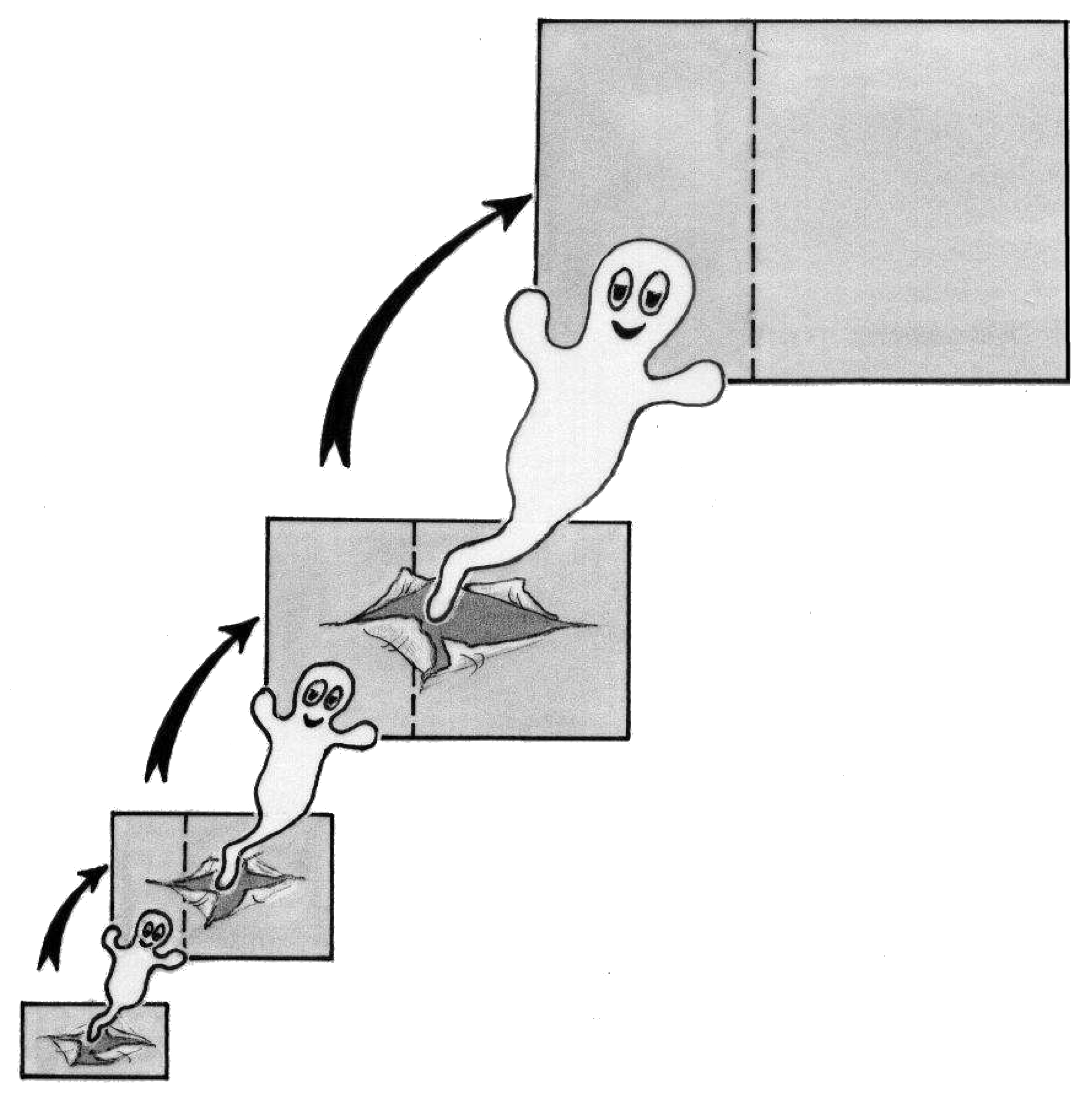
\includegraphics[width=10cm]{fantome}   
   \end{center}
   
   Par groupes, vous effectuerez les recherches, puis rendrez une fiche récapitulative où figureront votre raisonnement, la modélisation et les calculs effectués.
     
\end{enigme}

\vfill \hfill {\it\small D'après \og La résolution de problèmes mathématiques au collège \fg, MENJS, 2021}

\begin{corrige}
   On peut, par exemple, calculer les aires une par une jusqu'à obtenir $\umq{1,5} = \ummq{1500000}$. \\
   Le tableau ci-dessous récapitule la largeur et la longueur obtenue par chaque rectangle en mm ainsi que son aire en mm$^2$. \medskip
   
   \begin{tabular}{|c|c|c|c|}
      \hline
      Jour & Largeur & Longueur & Aire \\
      \hline
      0 & 2 & 3 & 6 \\
      \hline
      1 & 3 & 5 & 15 \\
      \hline
      2 & 5 & 8 & 40 \\
      \hline
      3 & 8 & 13 & 104 \\
      \hline
      4 & 13 & 22 & 286 \\
      \hline
      5 & 22 & 35 & 770 \\
      \hline
      6 & 35 & 57 & 1 995 \\
      \hline
      7 & 57 & 94 & 5 358 \\
      \hline
      8 & 94 & 151 & 14 194 \\
      \hline
      9 & 151 & 245 & 36 995 \\
      \hline
      10 & 245 & 396 & 97 020 \\
      \hline
      11 & 396 & 641 & 253 836 \\
      \hline
      12 & 641 & 1 037 & 664 717 \\
      \hline
      13 & 1 037 & 1 678 & 1 740 086 \\
      \hline
   \end{tabular}
   \medskip
   
   {\blue Il faudra 13 jours pour que l'aire du rectangle dépasse \umq{1,5}.}
\end{corrige}
      
